\documentclass[dvisvgm]{standalone}

\usepackage{tikz}
\usetikzlibrary {arrows.meta, positioning, automata}

\begin{document}

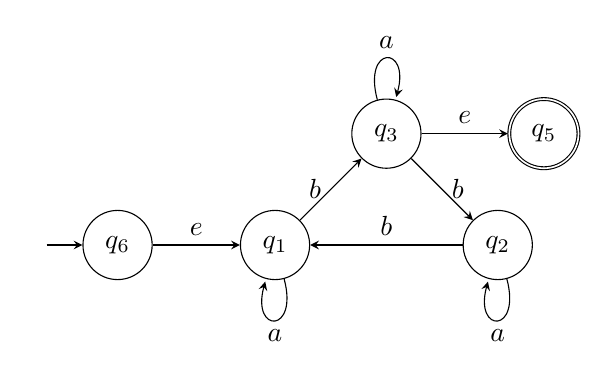
\begin{tikzpicture}[
    ->,
    >=stealth,
    node distance=2cm,
    initial text=$ $,
    on grid,
]

    \node[initial,   state]                    (A) {$q_6$};
    \node[           state, right =of A]       (B) {$q_1$};
    \node[           state, above right =of B] (C) {$q_3$};
    \node[           state, below right =of C] (D) {$q_2$};
    \node[accepting, state, right =of C]       (E) {$q_5$};

    \path
        (A) edge [above]      node {$e$}  (B)
        (B) edge [loop below] node {$a$}  (B)
        (B) edge [left]       node {$b$}  (C)
        (C) edge [loop above] node {$a$}  (C)
        (C) edge [right]      node {$b$}  (D)
        (D) edge [above]      node {$b$}  (B)
        (D) edge [loop below] node {$a$}  (D)
        (C) edge [above]      node {$e$}  (E)
    ;
\end{tikzpicture}

\end{document}